\documentclass[conference]{IEEEtran}
\IEEEoverridecommandlockouts
% The preceding line is only needed to identify funding in the first footnote. If that is unneeded, please comment it out.
\usepackage{cite}
\usepackage{amsmath,amssymb,amsfonts}
\usepackage{algorithmic}
\usepackage{graphicx}
\usepackage{textcomp}
\usepackage{xcolor}
\usepackage{tabularx}
\usepackage{multirow}
\usepackage{graphics} % for pdf, bitmapped graphics files
\usepackage{subfig}
\usepackage{subcaption}
\usepackage{hyperref}
\usepackage{academicons}
\usepackage{xcolor}
\def\BibTeX{{\rm B\kern-.05em{\sc i\kern-.025em b}\kern-.08em
		T\kern-.1667em\lower.7ex\hbox{E}\kern-.125emX}}
% Gráficas en MATLAB
\usepackage{tikz, pgfplots}
% Color Enlace
\definecolor{colorEnlace}{RGB}{0, 0, 0}
\hypersetup{
	colorlinks=true,
	linkcolor=colorEnlace,
	citecolor=colorEnlace,
	urlcolor=colorEnlace,
	pdfauthor={Davis Bremdow Salazar Roa},
	pdftitle={Introducción a LaTeX}
}
% Control 
\usepackage{amsmath}
\begin{document}
	
	\title{Generador Léxico - Tokenizador}
	\author{	
		\IEEEauthorblockN{Davis Bremdow Salazar Roa}
		\IEEEauthorblockA{Universidad Nacional de San Antonio Abad del Cusco}
		\textit{Escuela Profesional de Ingeniería Electrónica}\\
		\textit{Arquitectura de Microcontroladores y Microprocesadores}\\
		200353 \\\\
		Cusco, Perú
	}
	
	\maketitle
	
	\begin{abstract}
		Compilers are crucial in software development as they translate high-level programming code into machine code, optimizing it for different hardware architectures while identifying errors. A key part of compiler development is categorizing the code into basic structures using a tokenizer. In this process, object-oriented programming (OOP) in CSharp is used, with two main classes, **Token** and Lexer, to create the tokenization software. A state machine is implemented to classify tokens into categories like variables, assignments, and operators, though more tokens will be needed for comprehensive expression handling.
	\end{abstract}
	
	\begin{IEEEkeywords}
		Compilador, Generador de Léxico, Generador Sintáctico, Generador Sintáctico
	\end{IEEEkeywords}
	
	\section{Introducción}
		Los compiladores son herramientas esenciales en el desarrollo de software, ya que traducen el código fuente escrito en un lenguaje de programación de alto nivel a un lenguaje de bajo nivel o código máquina que puede ser entendido y ejecutado por la computadora. Esta conversión permite que los programas sean eficientes y optimizados para diferentes arquitecturas de hardware. Además, los compiladores ayudan a identificar errores en el código durante el proceso de traducción, mejorando así la calidad del software y facilitando el desarrollo de software.
	
	\section{Tokenizador de expresiones analíticas o ecuaciones}
	
	Una parte importante en el desarrollo de un compilador es la categorización del lenguaje de programación de alto a nivel en estructuras básicas mediante una etiqueta que las identifique, es por ello que un programa para este caso basado en la programación orientada a objetos sera de vital importancia para facilitar este proceso, brindando flexibilidad y escalamiento en el desarrollo del compilador.
	
	Para la creación del lenguaje de este programa se hizo uso del lenguaje CSharp y una de las metodologías de programación basada en la caracterización de objetos como entes virtuales, para este caso en concreto se definen 2 clases principales \textbf{Token} y \textbf{Lexer} las cuales se utilizaran para la creación del software de tokenización.
	
	Para la clasificación, subdivisión de caracteres para finalmente realizar la clasificación de cada token se definio una maquina de estados a nivel lógico y en la cual se definieron los estados necesarios para catalogar cada token en:
	\begin{itemize}
		\item Variable
		\item Asignación
		\item Operadores
	\end{itemize}
	
	Sin embargo para tener un mayor panorama en la creación de las expresiones será necesario agregar más categorías para la tokenización de elementos y en las cuales de forma necesaria se agrego un operador binario "!" (negación) y el reconocimiento de símbolos "(" y ")" para poder organizar las expresiones analíticas o matemáticas.
	
	Creando un estado adicional en la maquina de estados para este propósito, siendo este el código generado para tal reconocimiento y funcionamiento
	\begin{figure}[h]
		\centering
		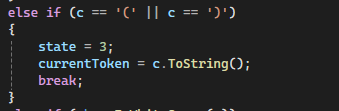
\includegraphics[width=0.5\textwidth]{media/con-simbolos}
		\caption{Condicional para el reconocimiento de simbolos}
		\label{fig:con-simbolos}
	\end{figure}
	
	\begin{figure}[h]
		\centering
		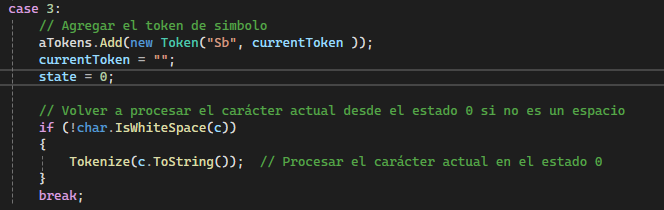
\includegraphics[width=0.5\textwidth]{media/simbolos-estado}
		\caption{Estado adicional para el reconocimiento de simbolos}
		\label{fig:simbolos-estado}
	\end{figure}
	
	Apreciándose en la \ref{fig:con-simbolos} las condicionales necesarias para el reconocimiento del símbolo agregado y en la figura \ref{fig:simbolos-estado} el código en el cual se define el nuevo estado para agregar/reconocer símbolos dentro del esquema de tokens generados.
	
	\section{Analizador Léxico}
	El analizador Léxico esta compuesto por 2 clases generales que nos permite tokenizar una determinada expresión dentro del lenguaje de alto nivel que se piensa ejecutar y en tal sentido y para ello se hace uso de las siguientes expresiones.
	
	\subsection{Token}
	La clase Token representa una unidad básica de información dentro del proceso de tokenización. Cada instancia de la clase contiene dos atributos: el tipo de token (por ejemplo, variable, operador, asignación) y el valor asociado (como una letra, un operador o un símbolo). Además, incluye un método para devolver una representación del token en formato de texto.
	
	Dentro de los métodos de la clase Token se puede rescatar el uso de la función GetTokenInfo que nos permite recuperar la representación del Token en forma de texto y la cual nos servirá para mostrar las salidas con todo los elementos tokenizados.
	
	\subsection{Lexer}
	La clase Lexer se encarga del proceso de tokenización, es decir, de dividir una expresión en tokens individuales. Utiliza una máquina de estados para recorrer cada carácter de una expresión, clasificando los tokens en categorías como operadores, variables, asignaciones o símbolos. Los tokens generados se almacenan en una lista, y la clase también incluye métodos para guardar estos tokens en un archivo o mostrarlos en pantalla.
	
	Dentro de la clase Lexer se pueden rescatar los siguientes métodos siendo el principal el método principal es Tokenize, que utiliza una máquina de estados para analizar una expresión y generar tokens. Además, hay métodos para guardar los tokens generados en un archivo (SaveTokensToFile) y para mostrarlos en pantalla (DisplayTokens), todos operando sobre la lista de tokens generados.
	
	
	
		
	
	\bibliographystyle{IEEEtran}
	\bibliography{biblio}
\end{document}
